\documentclass[]{article}
\usepackage{lmodern}
\usepackage{amssymb,amsmath}
\usepackage{ifxetex,ifluatex}
\usepackage{fixltx2e} % provides \textsubscript
\ifnum 0\ifxetex 1\fi\ifluatex 1\fi=0 % if pdftex
  \usepackage[T1]{fontenc}
  \usepackage[utf8]{inputenc}
\else % if luatex or xelatex
  \ifxetex
    \usepackage{mathspec}
  \else
    \usepackage{fontspec}
  \fi
  \defaultfontfeatures{Ligatures=TeX,Scale=MatchLowercase}
\fi
% use upquote if available, for straight quotes in verbatim environments
\IfFileExists{upquote.sty}{\usepackage{upquote}}{}
% use microtype if available
\IfFileExists{microtype.sty}{%
\usepackage{microtype}
\UseMicrotypeSet[protrusion]{basicmath} % disable protrusion for tt fonts
}{}
\usepackage[margin=1in]{geometry}
\usepackage{hyperref}
\hypersetup{unicode=true,
            pdftitle={Laborator Suplimentar},
            pdfborder={0 0 0},
            breaklinks=true}
\urlstyle{same}  % don't use monospace font for urls
\usepackage{color}
\usepackage{fancyvrb}
\newcommand{\VerbBar}{|}
\newcommand{\VERB}{\Verb[commandchars=\\\{\}]}
\DefineVerbatimEnvironment{Highlighting}{Verbatim}{commandchars=\\\{\}}
% Add ',fontsize=\small' for more characters per line
\usepackage{framed}
\definecolor{shadecolor}{RGB}{248,248,248}
\newenvironment{Shaded}{\begin{snugshade}}{\end{snugshade}}
\newcommand{\KeywordTok}[1]{\textcolor[rgb]{0.13,0.29,0.53}{\textbf{#1}}}
\newcommand{\DataTypeTok}[1]{\textcolor[rgb]{0.13,0.29,0.53}{#1}}
\newcommand{\DecValTok}[1]{\textcolor[rgb]{0.00,0.00,0.81}{#1}}
\newcommand{\BaseNTok}[1]{\textcolor[rgb]{0.00,0.00,0.81}{#1}}
\newcommand{\FloatTok}[1]{\textcolor[rgb]{0.00,0.00,0.81}{#1}}
\newcommand{\ConstantTok}[1]{\textcolor[rgb]{0.00,0.00,0.00}{#1}}
\newcommand{\CharTok}[1]{\textcolor[rgb]{0.31,0.60,0.02}{#1}}
\newcommand{\SpecialCharTok}[1]{\textcolor[rgb]{0.00,0.00,0.00}{#1}}
\newcommand{\StringTok}[1]{\textcolor[rgb]{0.31,0.60,0.02}{#1}}
\newcommand{\VerbatimStringTok}[1]{\textcolor[rgb]{0.31,0.60,0.02}{#1}}
\newcommand{\SpecialStringTok}[1]{\textcolor[rgb]{0.31,0.60,0.02}{#1}}
\newcommand{\ImportTok}[1]{#1}
\newcommand{\CommentTok}[1]{\textcolor[rgb]{0.56,0.35,0.01}{\textit{#1}}}
\newcommand{\DocumentationTok}[1]{\textcolor[rgb]{0.56,0.35,0.01}{\textbf{\textit{#1}}}}
\newcommand{\AnnotationTok}[1]{\textcolor[rgb]{0.56,0.35,0.01}{\textbf{\textit{#1}}}}
\newcommand{\CommentVarTok}[1]{\textcolor[rgb]{0.56,0.35,0.01}{\textbf{\textit{#1}}}}
\newcommand{\OtherTok}[1]{\textcolor[rgb]{0.56,0.35,0.01}{#1}}
\newcommand{\FunctionTok}[1]{\textcolor[rgb]{0.00,0.00,0.00}{#1}}
\newcommand{\VariableTok}[1]{\textcolor[rgb]{0.00,0.00,0.00}{#1}}
\newcommand{\ControlFlowTok}[1]{\textcolor[rgb]{0.13,0.29,0.53}{\textbf{#1}}}
\newcommand{\OperatorTok}[1]{\textcolor[rgb]{0.81,0.36,0.00}{\textbf{#1}}}
\newcommand{\BuiltInTok}[1]{#1}
\newcommand{\ExtensionTok}[1]{#1}
\newcommand{\PreprocessorTok}[1]{\textcolor[rgb]{0.56,0.35,0.01}{\textit{#1}}}
\newcommand{\AttributeTok}[1]{\textcolor[rgb]{0.77,0.63,0.00}{#1}}
\newcommand{\RegionMarkerTok}[1]{#1}
\newcommand{\InformationTok}[1]{\textcolor[rgb]{0.56,0.35,0.01}{\textbf{\textit{#1}}}}
\newcommand{\WarningTok}[1]{\textcolor[rgb]{0.56,0.35,0.01}{\textbf{\textit{#1}}}}
\newcommand{\AlertTok}[1]{\textcolor[rgb]{0.94,0.16,0.16}{#1}}
\newcommand{\ErrorTok}[1]{\textcolor[rgb]{0.64,0.00,0.00}{\textbf{#1}}}
\newcommand{\NormalTok}[1]{#1}
\usepackage{longtable,booktabs}
\usepackage{graphicx,grffile}
\makeatletter
\def\maxwidth{\ifdim\Gin@nat@width>\linewidth\linewidth\else\Gin@nat@width\fi}
\def\maxheight{\ifdim\Gin@nat@height>\textheight\textheight\else\Gin@nat@height\fi}
\makeatother
% Scale images if necessary, so that they will not overflow the page
% margins by default, and it is still possible to overwrite the defaults
% using explicit options in \includegraphics[width, height, ...]{}
\setkeys{Gin}{width=\maxwidth,height=\maxheight,keepaspectratio}
\IfFileExists{parskip.sty}{%
\usepackage{parskip}
}{% else
\setlength{\parindent}{0pt}
\setlength{\parskip}{6pt plus 2pt minus 1pt}
}
\setlength{\emergencystretch}{3em}  % prevent overfull lines
\providecommand{\tightlist}{%
  \setlength{\itemsep}{0pt}\setlength{\parskip}{0pt}}
\setcounter{secnumdepth}{5}
% Redefines (sub)paragraphs to behave more like sections
\ifx\paragraph\undefined\else
\let\oldparagraph\paragraph
\renewcommand{\paragraph}[1]{\oldparagraph{#1}\mbox{}}
\fi
\ifx\subparagraph\undefined\else
\let\oldsubparagraph\subparagraph
\renewcommand{\subparagraph}[1]{\oldsubparagraph{#1}\mbox{}}
\fi

%%% Use protect on footnotes to avoid problems with footnotes in titles
\let\rmarkdownfootnote\footnote%
\def\footnote{\protect\rmarkdownfootnote}

%%% Change title format to be more compact
\usepackage{titling}

% Create subtitle command for use in maketitle
\newcommand{\subtitle}[1]{
  \posttitle{
    \begin{center}\large#1\end{center}
    }
}

\setlength{\droptitle}{-2em}
  \title{Laborator Suplimentar}
  \pretitle{\vspace{\droptitle}\centering\huge}
  \posttitle{\par}
\subtitle{Mersul la întâmplare simplu}
  \author{}
  \preauthor{}\postauthor{}
  \date{}
  \predate{}\postdate{}

\usepackage{booktabs}
\usepackage{longtable}
\usepackage{framed,color}
\definecolor{shadecolor}{RGB}{248, 248, 248}
\definecolor{shadecolor1}{RGB}{216,225,235}
\definecolor{framecolor}{RGB}{108,123,13}

\ifxetex
  \usepackage{letltxmacro}
  \setlength{\XeTeXLinkMargin}{1pt}
  \LetLtxMacro\SavedIncludeGraphics\includegraphics
  \def\includegraphics#1#{% #1 catches optional stuff (star/opt. arg.)
    \IncludeGraphicsAux{#1}%
  }%
  \newcommand*{\IncludeGraphicsAux}[2]{%
    \XeTeXLinkBox{%
      \SavedIncludeGraphics#1{#2}%
    }%
  }%
\fi

\newenvironment{frshaded*}{%
  \def\FrameCommand{\fboxrule=\FrameRule\fboxsep=\FrameSep \fcolorbox{framecolor}{shadecolor1}}%
  \MakeFramed {\advance\hsize-\width \FrameRestore}}%
{\endMakeFramed}

\newenvironment{rmdblock}[1]
  {\begin{frshaded*}
  \begin{itemize}
  \renewcommand{\labelitemi}{
    \raisebox{-.7\height}[0pt][0pt]{
      {\setkeys{Gin}{width=2em,keepaspectratio}\includegraphics{images/icons/#1}}
    }
  }
  \item
  }
  {
  \end{itemize}
  \end{frshaded*}
  }
  
\newenvironment{rmdcaution}
  {\begin{rmdblock}{caution}}
  {\end{rmdblock}}
% \newenvironment{rmdinsight}
%   {\begin{rmdblock}{insight}}
%   {\end{rmdblock}}
\newenvironment{rmdexercise}
  {\begin{rmdblock}{exercise}}
  {\end{rmdblock}}
\newenvironment{rmdtip}
  {\begin{rmdblock}{tip}}
  {\end{rmdblock}}
  
  
%%%%%%%%%%%%%%%%%%%%%%%%%%%%%%%%%%%%%%%%%%%%%%%%%%%%%%%%%%%%%%%%%%%%%%%%%%%%%%%%%%%%%%%%%%%%%%%%%%%%%%%%%%%%%%%%%%%%%
%%%%%%%%%%% For insight block %%%%%%%%%%%%%%%%%%%%%%%%%%
\definecolor{shadecolor_insight}{RGB}{223,240,216}
\definecolor{framecolor_insight}{RGB}{136,193,137}

\newenvironment{frshaded_insight*}{%
  \def\FrameCommand{\fboxrule=\FrameRule\fboxsep=\FrameSep \fcolorbox{framecolor_insight}{shadecolor_insight}}%
  \MakeFramed {\advance\hsize-\width \FrameRestore}}%
{\endMakeFramed}

\newenvironment{rmdblock_insight}[1]
  {\begin{frshaded_insight*}
  \begin{itemize}
  \renewcommand{\labelitemi}{
    \raisebox{-.7\height}[0pt][0pt]{
      {\setkeys{Gin}{width=2em,keepaspectratio}\includegraphics{images/icons/#1}}
    }
  }
  \item
  }
  {
  \end{itemize}
  \end{frshaded_insight*}
  }
  
\newenvironment{rmdinsight}
  {\begin{rmdblock_insight}{insight}}
  {\end{rmdblock_insight}}
  
%%%%%%%%%%%%%%%%%%%%%%%%%%%%%%%%%%%%%%%%%%%%%%%%%%%%%%%%%%%%%%%%%%%%%%%%%%%%%%%%%%%%%%%%%%%%%%%%%%%%%%%%%%%%%%%%%%%%%
\usepackage{subfigure}
\usepackage{booktabs}
\usepackage{slashbox}
\usepackage{color}
%%%%%%%%%%%%%%%%%%%%%%%%%%%%%%%%%%%%%%%%%%%%%%%%%%%%%%%%%%%%%%%%%%%%%%%%%%%%%%%%%%%%%%%%%%%%%%%%%%%%%%%%%%%%%%%%%%%%%
%CITEVA DEFINITII
\def\om{\omega}
\def\Om{\Omega}
\def\et{\eta}
\def\td{\tilde{\delta}}
\def\m{{\mu}}
\def\n{{\nu}}
\def\k{{\kappa}}
\def\l{{\lambda}}
\def\L{{\Lambda}}
\def\g{{\gamma}}
\def\a{{\alpha}}
\def\e{{\varepsilon}}
\def\b{{\beta}}
\def\G{{\Gamma}}
\def\d{{\delta}}
\def\D{{\Delta}}
\def\t{{\theta}}
\def\s{{\sigma}}
\def\S{{\Sigma}}
\def\z{{\zeta}}
\def\qed{\hfill\Box}
\def\ds{\displaystyle}
\def\mc{\mathcal}
%%%%%%%%%%%%%%%%%%%%%%%%%%%%%%%%%%%%%%%%%%%%%%%%%%%%%%%%%%%%%%%%%%%%%%%%%%%%%%%%%%%%%%%%%%%%%%%%%%%%%%%%%%%%%%%%%%%%%%
\def\1{{\mathbf 1}}
\def\CC{{\mathbb C}}
\def\VV{{\mathbb V}}
\def\RR{{\mathbb R}}
\def\QQ{{\mathbb Q}}
\def\ZZ{{\mathbb Z}}
\def\PP{{\mathbb P}}
\def\EE{{\mathbb E}}
\def\NN{{\mathbb N}}
\def\FF{{\mathbb F}}
%\def\SS{{\mathbb S}}
\def\MA{{\mathcal A}}
\def\MO{{\mathcal O}}
\def\MF{{\mathcal F}}
\def\ME{{\mathcal E}}
\def\MR{{\mathcal R}}
\def\MB{{\mathcal B}}
\def\MM{{\mathcal M}}
\def\MN{{\mathcal N}}
\def\MU{{\mathcal U}}
\def\MP{{\mathcal P}}
\def\MS{{\mathcal S}}
\def\MBS{{\mathbf S}}
\def\MX{{\bm{ \mathscr X}}}

% independent sign
\newcommand\independent{\protect\mathpalette{\protect\independenT}{\perp}}
\def\independenT#1#2{\mathrel{\rlap{$#1#2$}\mkern2mu{#1#2}}}

\renewcommand{\figurename}{Fig.}

%%%%%%%%%%%%%%%%%%%%%%%%%%%%%%%%%%%%%%%%%%%%%%%%%%%%%%%%%%%%%%%%%%%%%%%%%%%%%%%%%%%%%%%%%%%%%%%%%%%%%%%%%%%%%%%%%%%%%
%Header and Footer
\usepackage{fancyhdr}

\pagestyle{fancy}
\fancyhf{}
\rhead{Universitatea din Bucure\c sti\\ Facultatea de Matematic\u a \c si Informatic\u a}
\lhead{\textit{Curs}: Statistic\u a\\ \textit{Instructori}: A. Am\u arioarei, S. Cojocea}
\rfoot{Pagina \thepage}
\lfoot{Grupele: 301, 311, 321}
%%%%%%%%%%%%%%%%%%%%%%%%%%%%%%%%%%%%%%%

\begin{document}
\maketitle

%%%%%%%%%%%%%%%%%%%%%%%%
\thispagestyle{fancy}

Obiectivul acestui laborator este de a rezolva câteva probleme ce țin de
mersul la întâmplare simplu cu ajutorul limbajului R.

\section{Ruina jucătorului}\label{ruina-jucatorului}

\begin{rmdexercise}
Un bărbat vrea să își cumpere un obiect (de exemplu o mașină sau o casă)
care costă \(N\) unități monetare. Să presupunem că el are economisit un
capital de \(0<k<N\) unități monetare și încearcă să câștige restul
jucând un joc de noroc cu managerul unei bănci. Jocul este următorul:
bărbatul aruncă o monedă echilibrată în mod repetatș dacă moneda pică
cap (\(H\)) atunci managerul îi dă o unitate monetară, în caz contrar
bărbatul plătește o unitate monetară bancii. Jocul continuă până când
unul din două evenimente se realizează: sau câștigă suma necesară și își
cumpără obiectul dorit sau pierde banii și ajunge la faliment. Ne
întrebăm care este probabilitatea să ajungă la faliment?
\end{rmdexercise}

Fie \(A\) evenimentul ca bărbatul să ajungă la ruină și \(B\)
evenimentul ca la prima aruncare moneda a picat cap. Atunci din formula
probabilității totale avem

\[
  \mathbb{P}_k(A) = \mathbb{P}_k(A|B)\mathbb{P}(B)+\mathbb{P}_k(A|B^c)\mathbb{P}(B^c)
\]

unde \(\mathbb{P}_k\) este probabilitatea calculată în funcție de
valoarea \(k\) a capitalului inițial al jucătorului. Să observăm că
\(\mathbb{P}_k(A|B)\) devine \(\mathbb{P}_{k+1}(A)\) deoarece dacă la
prima aruncare avem cap atunci capitalul inițial a crescut la \(k+1\).
În mod similar, dacă la prima aruncare am obținut coadă atunci
\(\mathbb{P}_k(A|B^c) = \mathbb{P}_{k-1}(A)\). Notând cu
\(p_k = \mathbb{P}_k(A|B)\) obținem următoarea ecuație

\[
  p_k = \frac{1}{2}p_{k+1} + \frac{1}{2}p_{k-1},
\]

cu valorile inițiale \(p_0=1\) (dacă jucătorul a pornit cu un capital
inițial nul atunci el este în faliment) și respectiv \(p_N=0\) (dacă
jucătorul are din start suma necesară pentru a achiziționa obiectul
dorit atunci nu mai are loc jocul).

O simulare a jocului pentru \(N = 50\) și \(k = 5\) este prezentată de
următoarea funcție:

\begin{Shaded}
\begin{Highlighting}[]
\NormalTok{ruina =}\StringTok{ }\ControlFlowTok{function}\NormalTok{(N, k)\{}
\NormalTok{  flag =}\StringTok{ }\OtherTok{TRUE}

\NormalTok{  joc =}\StringTok{ }\DecValTok{0}
\NormalTok{  capital =}\StringTok{ }\NormalTok{k}
\NormalTok{  y =}\StringTok{ }\NormalTok{capital}
  
  \ControlFlowTok{while}\NormalTok{(flag)\{}
\NormalTok{    x =}\StringTok{ }\DecValTok{2}\OperatorTok{*}\KeywordTok{rbinom}\NormalTok{(}\DecValTok{1}\NormalTok{,}\DecValTok{1}\NormalTok{,}\FloatTok{0.5}\NormalTok{)}\OperatorTok{-}\DecValTok{1}
    
\NormalTok{    capital =}\StringTok{ }\NormalTok{capital }\OperatorTok{+}\StringTok{ }\NormalTok{x}
\NormalTok{    y =}\StringTok{ }\KeywordTok{c}\NormalTok{(y, capital)}
    
\NormalTok{    joc =}\StringTok{ }\NormalTok{joc }\OperatorTok{+}\StringTok{ }\DecValTok{1}
    
    \ControlFlowTok{if}\NormalTok{ (capital }\OperatorTok{==}\StringTok{ }\DecValTok{0} \OperatorTok{||}\StringTok{ }\NormalTok{capital }\OperatorTok{==}\StringTok{ }\NormalTok{N)\{}
\NormalTok{      flag =}\StringTok{ }\OtherTok{FALSE}
\NormalTok{    \}}
\NormalTok{  \}}
  
  \KeywordTok{return}\NormalTok{(y) }\CommentTok{# daca am 0 este ruina altfel este succes}
\NormalTok{\}}
\end{Highlighting}
\end{Shaded}

\begin{center}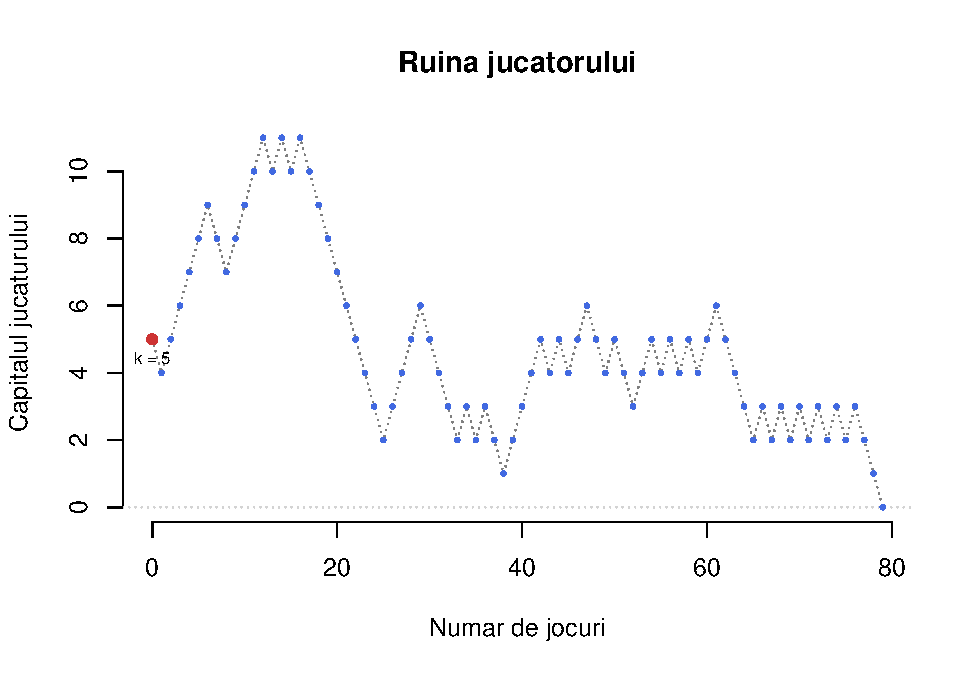
\includegraphics{Lab_Suplimentar_files/figure-latex/unnamed-chunk-4-1} \end{center}

Dacă definim \(b_k = p_k - p_{k-1}\) pentru \(k\geq 1\) atunci
\(b_k = b_{k-1}\), \(\forall k\geq2\). Prin urmare \(b_k = b_1\) și
\(p_k = b_1+p_{k-1} = kb_1+p_0\). Observând că
\(b_1+\cdots+b_N=p_N-p_0=-1\) deducem că \(b_1=-\frac{1}{N}\) iar
\(p_k=1-\frac{k}{N}\).

Dorim să repetăm experimentul de \(M = 1000\) de ori (pentru valorile
inițiale \(N = 50\) și \(k = 5\)) și ne interesăm de câte ori jucătorul
a ajuns la faliment.

\begin{Shaded}
\begin{Highlighting}[]
\NormalTok{N =}\StringTok{ }\DecValTok{50}
\NormalTok{k =}\StringTok{ }\DecValTok{5}
\NormalTok{M =}\StringTok{ }\DecValTok{1000}
\CommentTok{# Obs. - rezultatul functiei ruina trebuie modificat}
\NormalTok{joc =}\StringTok{ }\KeywordTok{replicate}\NormalTok{(M, }\KeywordTok{ruina}\NormalTok{(N, k)) }\CommentTok{# repeta functia de M ori }

\NormalTok{proba_ruina =}\StringTok{ }\KeywordTok{sum}\NormalTok{(joc }\OperatorTok{==}\StringTok{ }\DecValTok{0}\NormalTok{)}\OperatorTok{/}\NormalTok{M }
\end{Highlighting}
\end{Shaded}

Am obținut că probabilitatea empirică de faliment este 0.9 iar cea
teoretică este 0.9.

\section{Aruncatul cu banul}\label{aruncatul-cu-banul}

\begin{rmdexercise}
O monedă are probabilitatea să pice cap \(p\) și să pice coadă \(q\)
astfel ca \(p+q=1\). Moneda este aruncată succesiv și independent până
când evenimentul \(A\), am obținut două capete unul după altul sau două
cozi una după alta, s-a realizat. Determinați numărul mediu de aruncări
necesare realizării evenimentului \(A\).
\end{rmdexercise}

Vom prezenta două soluții pentru acest exercițiu. În prima soluție vom
începe prin a calcula funcția de masă pentru variabila care descrie
experimentul și apoi vom calcula media. În cea de-a doua soluție vom
calcula media cu ajutorul condiționării.

Fie \(X\) variabila aleatoare care reprezintă numărul de aruncări
necesare pentru ca evenimentul \(A\) să se realizeze (numărul de
aruncări necesare obținerii a \(2\) capete unul după altul sau a \(2\)
cozi una după alta) și \(X_i\in\{H,T\}\) variabila aleatoare care
descrie rezultatul obținut la cea de-a i-a aruncare. Evenimentul
\(\{X=n\}\) poate fi exprimat ca reuniunea dintre \(A_n\) și \(B_n\),
unde \(A_n\) reprezintă evenimentul să obținem două capete consecutive
pentru prima oară la cea de-a \(n\)-a aruncare iar \(B_n\) este
evenimentul să obținem două cozi consecutive la a \(n\)-a aruncare.

Se poate observa cu ușurință că un eveniment elementar din \(A_n\) are
forma \(\omega = \underbrace{\cdots}_{n-2} HH\) și se poate determina în
întregime datorită faptului că în primele \(n-2\) aruncări nu putem avea
două realizări consecutive. În plus dacă \(n = 2k+1\) atunci

\[
  \mathbb{P}(A_{2k+1}) = \mathbb{P}(X_1 = T, X_2 = H, \cdots, X_{2k-1}=T, X_{2k} = H, X_{2k+1} = H) \overset{indep.}{=} (pq)^kp 
\]\\
iar dacă \(n=2k+2\) atunci

\[
  \mathbb{P}(A_{2k+2}) = \mathbb{P}(X_1 = H, X_2 = T, \cdots, X_{2k}=T, X_{2k+1} = H, X_{2k+2} = H) \overset{indep.}{=} (pq)^kp^2 
\]

În mod similar se poate calcula probabilitatea evenimentului \(B_n\)
pentru \(n=2k+1\)

\[
  \mathbb{P}(B_{2k+1}) = \mathbb{P}(X_1 = H, X_2 = T, \cdots, X_{2k-1} = H, X_{2k} = T, X_{2k+1} = T) \overset{indep.}{=} (pq)^kq 
\]

și respectiv \(n=2k+2\)

\[
  \mathbb{P}(B_{2k+2}) = \mathbb{P}(X_1 = T, X_2 = H, \cdots, X_{2k} = H, X_{2k+1} = T, X_{2k+2} = T) \overset{indep.}{=} (pq)^kq^2 
\]

Cum \(\mathbb{P}(X=n) = \mathbb{P}(A_n) + \mathbb{P}(B_n)\) deducem că

\[
  \mathbb{P}(X=n) =\left\{\begin{array}{ll}
      (pq)^{\frac{n-1}{2}}, & \text{$n$ impar}\\
      (pq)^{\frac{n-2}{2}}(p^2+q^2), & \text{$n$ par}
  \end{array}\right.
\]

Următoarea funcție simulează evenimentul din enunțul problemei:

\begin{Shaded}
\begin{Highlighting}[]
\NormalTok{flip_coins =}\StringTok{ }\ControlFlowTok{function}\NormalTok{(p)\{}
  
\NormalTok{  flip =}\StringTok{ }\KeywordTok{sample}\NormalTok{(}\KeywordTok{c}\NormalTok{(}\StringTok{"H"}\NormalTok{, }\StringTok{"T"}\NormalTok{), }\DecValTok{1}\NormalTok{, }\DataTypeTok{prob =} \KeywordTok{c}\NormalTok{(p, }\DecValTok{1}\OperatorTok{-}\NormalTok{p))}
  
\NormalTok{  nflips =}\StringTok{ }\DecValTok{1}
\NormalTok{  flag =}\StringTok{ }\OtherTok{TRUE}
  
  \ControlFlowTok{while}\NormalTok{(flag)\{}
\NormalTok{    x =}\StringTok{ }\KeywordTok{sample}\NormalTok{(}\KeywordTok{c}\NormalTok{(}\StringTok{"H"}\NormalTok{, }\StringTok{"T"}\NormalTok{), }\DecValTok{1}\NormalTok{, }\DataTypeTok{prob =} \KeywordTok{c}\NormalTok{(p, }\DecValTok{1}\OperatorTok{-}\NormalTok{p))}
    
\NormalTok{    nflips =}\StringTok{ }\NormalTok{nflips }\OperatorTok{+}\StringTok{ }\DecValTok{1}
    
    \ControlFlowTok{if}\NormalTok{ (flip }\OperatorTok{==}\StringTok{ }\NormalTok{x)\{}
\NormalTok{      flag =}\StringTok{ }\OtherTok{FALSE}
\NormalTok{    \}}
    
\NormalTok{    flip =}\StringTok{ }\NormalTok{x}
\NormalTok{  \}}
  
  \KeywordTok{return}\NormalTok{(nflips)}
\NormalTok{\}}

\KeywordTok{flip_coins}\NormalTok{(}\FloatTok{0.2}\NormalTok{)}
\NormalTok{[}\DecValTok{1}\NormalTok{] }\DecValTok{3}
\end{Highlighting}
\end{Shaded}

Înainte de a calcula media ne propunem să repetăm de \(N = 10000\) de
ori experimentul (pentru \(p=0.3\)) și să comparăm rezultatul empiric cu
cel teoretic.

\begin{Shaded}
\begin{Highlighting}[]
\NormalTok{N =}\StringTok{ }\DecValTok{10000}
\NormalTok{p =}\StringTok{ }\FloatTok{0.3}

\NormalTok{rez_flips =}\StringTok{ }\KeywordTok{replicate}\NormalTok{(N, }\KeywordTok{flip_coins}\NormalTok{(p))}
\end{Highlighting}
\end{Shaded}

Rezultatele sunt incluse în tabelul de mai jos:

\begin{longtable}[]{@{}ccc@{}}
\toprule
n & Empiric & Teoretic\tabularnewline
\midrule
\endhead
2 & 0.5760 & 0.58000\tabularnewline
3 & 0.2110 & 0.21000\tabularnewline
4 & 0.1245 & 0.12180\tabularnewline
5 & 0.0434 & 0.04410\tabularnewline
6 & 0.0255 & 0.02558\tabularnewline
7 & 0.0100 & 0.00926\tabularnewline
8 & 0.0059 & 0.00537\tabularnewline
9 & 0.0016 & 0.00194\tabularnewline
10 & 0.0014 & 0.00113\tabularnewline
11 & 0.0004 & 0.00041\tabularnewline
12 & 0.0002 & 0.00024\tabularnewline
13 & 0.0001 & 0.00009\tabularnewline
\bottomrule
\end{longtable}

Pentru a calcula media avem

\[
  \mathbb{E}[X] = \sum_{n=2}^{\infty}n\mathbb{P}(X=n) 
\]

iar dacă seriile \(\sum_{k=1}^{\infty}(2k+1)\mathbb{P}(X=2k+1)\) și
\(\sum_{k=0}^{\infty}(2k+2)\mathbb{P}(X=2k+2)\) sunt convergente atunci
putem scrie

\[
  \mathbb{E}[X] = \sum_{n=2}^{\infty}n\mathbb{P}(X=n) = \sum_{k=1}^{\infty}(2k+1)\mathbb{P}(X=2k+1) + \sum_{k=0}^{\infty}(2k+2)\mathbb{P}(X=2k+2).
\]

Se poate arăta cu ușurință că

\[
  \sum_{k=1}^{\infty}(2k+1)\mathbb{P}(X=2k+1) = 2\sum_{k=1}^{\infty}(k+1)(pq)^k - \sum_{k=1}^{\infty}(pq)^k = \frac{pq(3-pq)}{(1-pq)^2}
\]

și

\[
  \sum_{k=0}^{\infty}(2k+2)\mathbb{P}(X=2k+2) = 2(p^2+q^2)\sum_{k=0}^{\infty}(k+1)(pq)^k = \frac{2(p^2+q^2)}{(1-pq)^2}
\]

de unde concluzionăm că
\(\mathbb{E}[X] = \frac{pq(3-pq)}{(1-pq)^2} + \frac{2(p^2+q^2)}{(1-pq)^2} = \frac{2+pq}{1-pq}\).

O a doua soluție pentru determinarea mediei este bazată pe condiționare.
Fie \(H_k\) și respectiv \(T_k\) evenimentele prin care capul respectiv
coada a apărut la cea de-a \(k\)-a aruncare și \(\mathbb{P}(H_k) = p\)
iar \(\mathbb{P}(T_k) = q\). Din formula probabilității totale, avem că

\[
  \mathbb{E}[X] = \mathbb{E}[X|H_1]\mathbb{P}(H_1) + \mathbb{E}[X|T_1]\mathbb{P}(T_1) = p\mathbb{E}[X|H_1] + q\mathbb{E}[X|T_1].
\]

Mai mult,

\[
  \mathbb{E}[X|H_1] = p\mathbb{E}[X|H_1\cap H_2] + q\mathbb{E}[X|H_1\cap T_2]
\]

și cum \(\mathbb{E}[X|H_1\cap H_2] = 2\) (evenimentul \(A\) s-a realizat
la a doua aruncare) iar
\(\mathbb{E}[X|H_1\cap T_2] = 1 + \mathbb{E}[X|T_1]\) (dacă jocul nu
este gata doar ultima aruncare este importantă) obținem că

\[
  \mathbb{E}[X|H_1] = 2p + q(1+\mathbb{E}[X|T_1]).
\]

În mod similar găsim
\(\mathbb{E}[X|T_1] = 2q + p(1+\mathbb{E}[X|H_1])\). Rezolvând sistemul
de două ecuații cu două necunoscute obținem soluțiile
\(\mathbb{E}[X|H_1] = \frac{2+q^2}{1-pq}\) și
\(\mathbb{E}[X|T_1] = \frac{2+p^2}{1-pq}\) de unde media este
\(\mathbb{E}[X] = \frac{2+pq}{1-pq}\).

Putem verifica numeric dacă formula pe care am gasit-o este corectă.
Pentru aceasta vom repeta experimentul (\(p = 0.3\)) de \(N = 10000\) de
ori.

Obținem că media empirică este 2.807 iar cea teoretică este 2.797.

\section{Principiul reflexiei și problema
scrutinului}\label{principiul-reflexiei-si-problema-scrutinului}

Să presupunem că avem \(n\) elemente
\(\epsilon_1, \ldots, \epsilon_n\in\{-1,+1\}\) astfel încât \(p\) dintre
ele iau valori de \(+1\) și \(q\) dintre ele iau valori de \(-1\)
(\(n = p + q\)). Sumele parțiale
\(s_k = \epsilon_1+\epsilon_2+\cdots+\epsilon_k\) reprezintă diferența
dintre numărul de elemente de \(+1\) și de elemente de \(-1\) în primele
\(k\) elemente. Observăm că

\[
  s_k-s_{k-1}=\epsilon_k=\pm 1,\quad s_0 = 0,\quad s_n = p-q.
\]

Din punct de vedere geometric, \(n\)-uplul
\((\epsilon_1,\ldots,\epsilon_n)\) poate fi reprezentat cu ajutorul unei
linii poligonale ce pleacă din origine și ajunge în punctul de
coordonate \((n,s_n)\), panta fiecărui segment de lungime \(1\) este
dată de \(\epsilon_k\) (\(+1\) NE și \(-1\) SE). Linia poligonală
\((s_1,\ldots,s_n)\) are al \(k\)-lea punct de abscisă \(k\) și ordonată
\(s_k\).

\begin{center}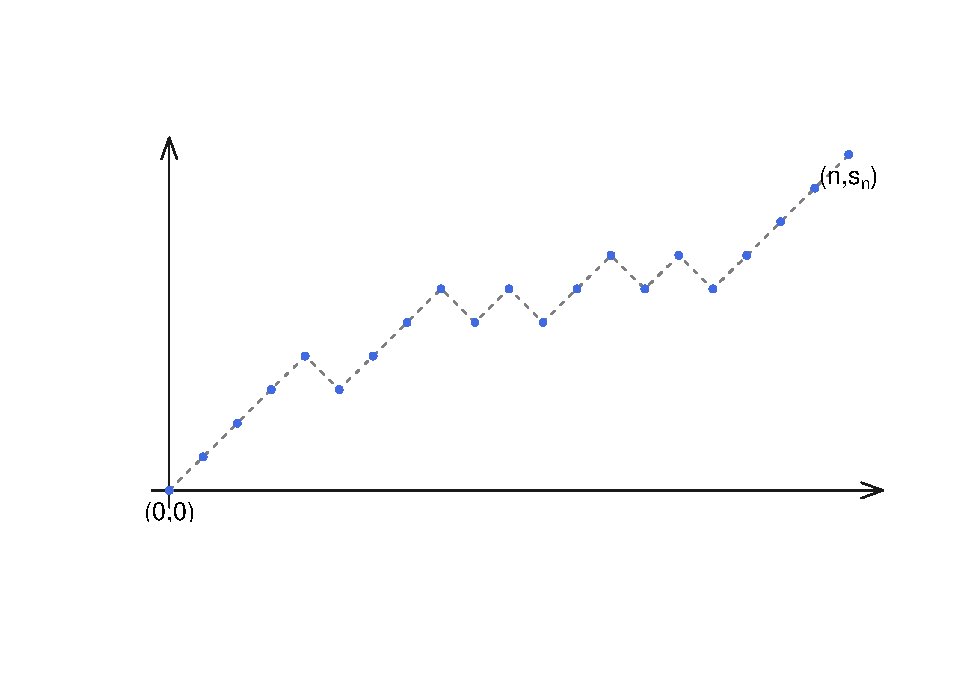
\includegraphics{Lab_Suplimentar_files/figure-latex/unnamed-chunk-12-1} \end{center}

Dacă \(n\) și \(x\) sunt numere naturale nenule astfel ca \(n = p+q\) și
\(x = p-q\), \(p, q\in\mathbb{N}\) atunci numărul de linii poligonale
(în sensul de mai sus) din origine către punctul \((n,x)\) este dat de

\[
  N_{n,x} = \binom{p+q}{p}.
\]

\begin{rmdexercise}
Să presupunem că în turul doi al alegerilor prezidențiale din 2019
participă doi candidați, \(P\) și \(Q\). Dacă voturile sunt date de
manieră independentă cu probabilitatea de \(\frac{1}{2}\) pentru fiecare
candidat și candidatul \(P\) primește \(p\) voturi iar candidatul \(Q\)
primește \(q\) voturi astfel ca \(P\) să câștige (\(p>q\)), atunci să se
calculeze probabilitatea ca pe tot parcursul numărării voturilor
candidatul \(P\) să fi avut mai multe voturi decât candidatul \(Q\).
\end{rmdexercise}

Problema scrutinului (propusă și rezolvată de Whitworth în
1878\footnote{Soluția a fost publicată în cartea
  \href{https://ia902307.us.archive.org/21/items/choicechance00whitrich/choicechance00whitrich.pdf}{Choice
  and chance} în 1886. În 1887
  \href{http://webspace.ship.edu/msrenault/ballotproblem/French\%20Bertrand.pdf}{Joseph
  Bertrand} a propus o formă mai generală a problemei care a fost
  rezolvată de către
  \href{http://webspace.ship.edu/msrenault/ballotproblem/French\%20Andre.pdf}{Désiré
  André} cu ajutorul principiului reflexiei.}) poate fi interpretată
geometric prin intermediul unei linii poligonale de lungime \(p+q\) în
care pantele fiecărui segment reprezintă opțiunea votului pentru unul
din cei doi candidați: \(\epsilon_k = +1\) dacă al \(k\)-lea vot a fost
pentru candidatul \(P\) și \(\epsilon_k = -1\) dacă al \(k\)-lea vot a
fost pentru candidatul \(Q\). În mod similar, dată fiind o linie
poligonală care pleacă din origine și ajunge în punctul \((p+q, p-q)\),
aceasta poate reprezenta parcursul unui scrutin în care cei doi
candidați vor avea la final \(p\) și respectiv \(q\) voturi.

Conform notațiilor precedente, putem observa că \(s_k\) reprezintă
numărul voturilor cu care candidatul \(P\) conduce (sau este în urmă)
imediat după cel de-al \(k\)-lea vot. Astfel cerința problemei se poate
traduce în modul următor: candidatul \(P\) conduce pe tot parcursul
procesului de votare dacă și numai dacă \(s_1>0, s_2>0,\ldots, s_n>0\)
(linia poligonală se află tot timpul deasupra axei absciselor).

Soluția problemei se bazează pe următorul rezultat, numit
\emph{principiul reflexiei}. Acesta spune că numărul de traiectorii
(linii poligonale în sensul descris mai sus) de la punctul de coordonate
\((x,y)\) la punctul de coordonate \((x',y')\), cu \(x'>x\geq0\),
\(y>0\) și \(y'>0\), care intersectează axa absciselor este egal cu
numărul de traiectorii de la punctul de coordonate \((x,-y)\) la punctul
de coordonate \((x',y')\).

\begin{center}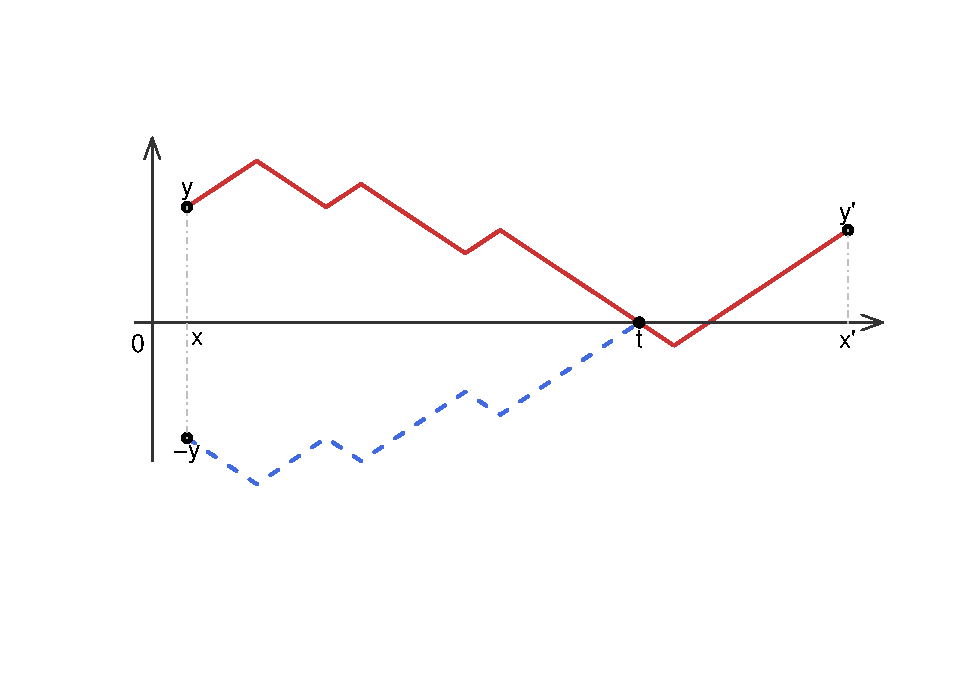
\includegraphics{Lab_Suplimentar_files/figure-latex/unnamed-chunk-14-1} \end{center}

Pentru a verifica această afirmație, fie
\((s_x = y, s_{x+1},\ldots,s_{x'} = y')\) o linie poligonală
(\(s_k-s_{k-1}=\pm 1\), \(k\in\{x,x+1,\ldots, x'\}\)) de la punctul
\((x,y)\) la punctul \((x',y')\) care să intersecteze axa absciselor și
fie \(t\) abscisa primului punct de intersecție (alegem \(t\) astfel
încât \(s_x>0,\ldots,s_{t-1}>0\) și \(s_t = 0\) - a se vedea figura).
Prin urmare
\((-s_x = -y, -s_{x+1},\ldots,-s_{t-1},0,s_{t+1},\ldots,s_{x'} = y')\)
este o linie poligonală de la punctul \((x,-y)\) la punctul \((x',y')\)
care intersectează axa absciselor pentru prima oară în punctul
\((t,0)\). Cum secțiunea \((s_x, s_{x+1},\ldots,s_{t-1},0)\) este
reflexia secțiunii \((-s_x, -s_{x+1},\ldots,-s_{t-1},0)\), deducem că
putem construi o bijecție de la mulțimea liniilor poligonale dintre
\((x,y)\) și \((x',y')\) la mulțimea liniilor poligonale dintre
\((x,-y)\) și \((x',y')\).

Vom arăta că numărul de linii poligonale care pleacă din origine și
ajung în punctul de coordonate \((p+q,p-q)\) verificând
\(s_1>0, s_2>0,\ldots, s_n>0\) este dat de formula:

\[
  N = \frac{p-q}{p+q}\binom{p+q}{p}.
\]

Pentru a verifica această formulă să observăm că numărul de linii
poligonale de la punctul \((0,0)\) la punctul \((n,x)\) (\(n = p+q\) și
\(x = p-q\)) care verifică \(s_1>0, s_2>0,\ldots, s_n>0\) coincide cu
numărul de traiectorii de la \((1,1)\) la \((n,x)\). Acest număr
reprezintă diferența dintre numărul de traiectorii din origine la
punctul \((n-1,x-1)\) (translatăm toate punctele spre stânga și în jos
cu o unitate), \(N_{n-1,x-1}\), mai puțin acele traiectorii care
intersectează axa absciselor. Folosind principiul reflexiei, numărul de
traiectorii care pornesc din \((1,1)\) și ajung în \((n,x)\)
intersectând axa absciselor este egal cu numărul de traiectorii care
pleacă din \((1,-1)\) și ajung în \((n,x)\), care este egal cu
\(N_{n-1,x+1}\) (translatăm spre stânga și în sus cu o unitate). Prin
urmare avem

\[
  N = N_{n-1,x-1} - N_{n-1,x+1} = \binom{p+q-1}{p-1} - \binom{p+q-1}{p} = \frac{p-q}{p+q}\binom{p+q}{p}.
\]

Probabilitatea căutată devine astfel
\(\frac{N_{n-1,x-1} - N_{n-1,x+1}}{N_{n,x}} = \frac{p-q}{p+q}\).

Pentru a verifica numeric rezultatul obținut să considerăm următoarea
funcție care simulează scrutin-ul pentru cei doi candidați:

\begin{Shaded}
\begin{Highlighting}[]
\NormalTok{scrutin =}\StringTok{ }\ControlFlowTok{function}\NormalTok{(sd)\{}
  \KeywordTok{set.seed}\NormalTok{(sd)}
  \CommentTok{# generam voturile}
\NormalTok{  vectscrutin =}\StringTok{ }\KeywordTok{sample}\NormalTok{(}\KeywordTok{c}\NormalTok{(}\KeywordTok{rep}\NormalTok{(}\StringTok{"P"}\NormalTok{,p),}\KeywordTok{rep}\NormalTok{(}\StringTok{"Q"}\NormalTok{,q)))}
  \CommentTok{# transformam in +-1 }
\NormalTok{  vectscrutin =}\StringTok{ }\DecValTok{2}\OperatorTok{*}\NormalTok{(vectscrutin }\OperatorTok{==}\StringTok{ "P"}\NormalTok{) }\OperatorTok{-}\StringTok{ }\DecValTok{1}
  \CommentTok{# calculam s_k}
\NormalTok{  s =}\StringTok{ }\KeywordTok{cumsum}\NormalTok{(vectscrutin)}
  \CommentTok{# returnam daca avem sau nu indeplinita conditia}
  \KeywordTok{sum}\NormalTok{(s}\OperatorTok{>}\DecValTok{0}\NormalTok{) }\OperatorTok{==}\StringTok{ }\NormalTok{p}\OperatorTok{+}\NormalTok{q}
\NormalTok{\}}
\end{Highlighting}
\end{Shaded}

Considerând \(p = 50\) și \(q = 35\) și repetând experimentul de
\(M = 100000\) de ori obținem că probabilitatea empirică este 0.1769 iar
cea teoretică este 0.1765.

\section{Legea arcsinus-ului}\label{legea-arcsinus-ului}

\begin{rmdexercise}
Să presupunem că aruncăm cu banul de \(100\) de ori și că înregistrăm la
fiecare aruncare numărul de capete și numărul de cozi. Definim
\emph{ultima egalitate} ca fiind ultima aruncare în care numărul de
capete este egal cu numărul de cozi (deci ia valori de la \(0\) la
\(100\)). Ne propunem să scriem un program care să determine locația
ultimei egalități în jocul de noroc descris.
\end{rmdexercise}

Vom începe prin a transpune problema în limbaj matematic\footnote{Această
  problemă este preluată din cartea lui W. Feller \emph{Introduction to
  probability and its applications}, vol I, 1968, capitolul III.}. Fie
\((X_n)_n\) un șir de variabile aleatoare independente ce iau valori în
mulțimea \(\{+1,-1\}\) cu probabilitatea \(p = \frac{1}{2}\) (aruncăm cu
banul și ne deplasăm la dreapta sau la stânga în funcție de rezultatul
aruncării) și fie \(S_n = X_1 + \cdots + X_n\). Putem interpreta șirul
\(S_1,S_2,\ldots,S_n\) geometric, ca și în cazul problemei scrutinului,
cu ajutorul unei linii poligonale cu segmentele
\((k-1, S_{k-1})\to(k, S_k)\). Fie \(L_{2n}\) variabila aleatoare care
ne dă timpul ultimei întoarceri în origine a unui mers la întâmplare de
lungime \(2n\) (de ce avem \(2n\)?), cu alte cuvinte

\[
  L_{2n} = \sup\{m\leq 2n\,|\,S_m = 0\}.
\]

Variabila \(L_{2n}\) este variabila care descrie \emph{ultima egalitate}
din enunțul problemei și ne propunem să găsim repartiția acestei
variabile aleatoare. Observăm că

\begin{align*}
  \mathbb{P}(L_{2n} = 2k) &= \mathbb{P}(S_{2k} = 0, S_{2k+1}\neq 0, \ldots, S_{2n}\neq 0)\\
                          &= \mathbb{P}(S_{2k} = 0)\mathbb{P}(S_{2k+1}\neq 0, \ldots, S_{2n}\neq 0|S_{2k} = 0).
\end{align*}

O realizare a variabilei \(L_{100}\), în contextul problemei atunci când
\(n = 50\) este ilustrată în figura următoare.

\begin{center}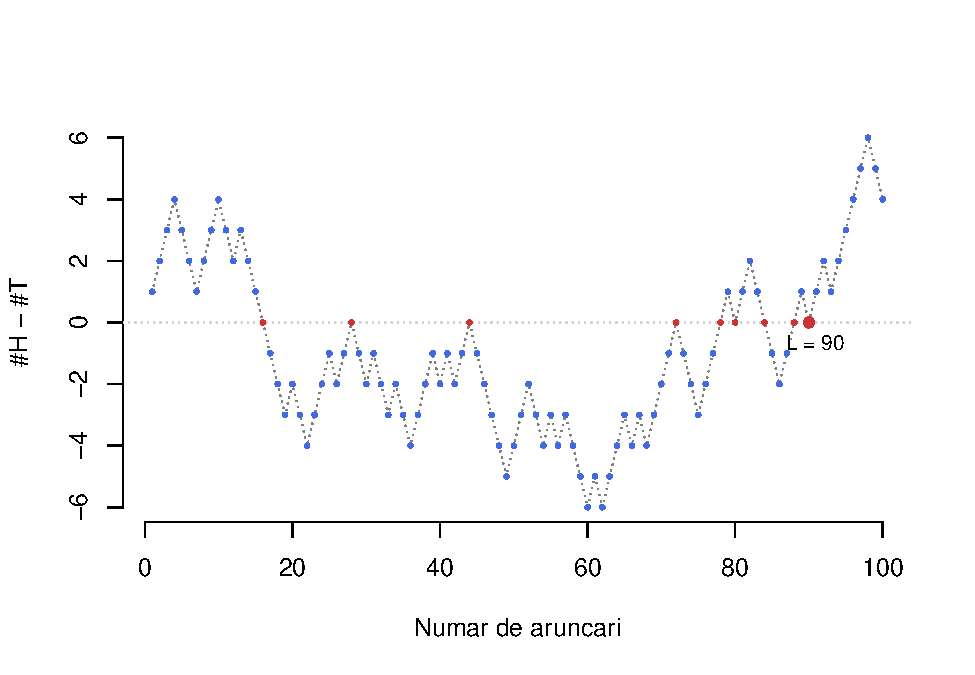
\includegraphics{Lab_Suplimentar_files/figure-latex/unnamed-chunk-18-1} \end{center}

Am văzut, în problema scrutinnului, că \(\mathbb{P}(S_n=m)\) este
\(\frac{N_{n,m}}{2^n}\) (numărul de linii poligonale din origine până în
punctul \((n,m)\) supra numărul total de linii poligonale cu \(n\)
puncte) de unde

\[
  \mathbb{P}(S_n=m) = \binom{n}{\frac{n+m}{2}}2^{-n},
\] unde folosim convenția că \(\binom{n}{\frac{n+m}{2}} = 0\) dacă
\(\frac{n+m}{2}\) nu este un întreg între \(0\) și \(n\). Astfel deducem
că \(\mathbb{P}(S_{2n} = 0) = \binom{2n}{n}2^{-2n}\).

Vom arăta că pentru un mers la întâmplare care începe din origine are
loc relația

\[
  \mathbb{P}(S_1\neq 0, S_2\neq 0, \ldots, S_{2n}\neq 0) = \mathbb{P}(S_{2n}=0)
\]

și cum \(X_i\) sunt independente (fiecare aruncare se face de manieră
independentă) atunci probabilitatea condiționată
\(\mathbb{P}(S_{2k+1}\neq 0, \ldots, S_{2n}\neq 0|S_{2k} = 0)\) este
egală cu probabilitatea ca un mers la întâmplare de lungime \(2n-2k\),
care pornește din origine, să nu mai viziteze niciodată originea în cei
\(2n-2k\) pași sau

\[
  \mathbb{P}(S_{2k+1}\neq 0, \ldots, S_{2n}\neq 0|S_{2k} = 0) = \mathbb{P}(S_{2n-2k}=0).
\]

Prin urmare avem relația
\(\mathbb{P}(L_{2n} = 2k) = \mathbb{P}(S_{2k}=0)\mathbb{P}(S_{2n-2k}=0)\).
Pentru ca demonstrația să fie completă rămâne să verificăm că

\[
  \mathbb{P}(S_1\neq 0, S_2\neq 0, \ldots, S_{2n}\neq 0) = \mathbb{P}(S_{2n}=0).
\]

Cum originea nu mai este vizitată în cei \(2n\) pași atunci sau
\(S_j>0\) sau \(S_j<0\) pentru toți \(j\in\{1,2,\ldots,n\}\). Din
simetrie, aceste alternative au aceeași probabilitate deci

\[
  \mathbb{P}(S_1\neq 0, S_2\neq 0, \ldots, S_{2n}\neq 0) = 2 \mathbb{P}(S_1> 0, S_2> 0, \ldots, S_{2n}> 0)
\]

și aplicând problema scrutinului (linia poligonală se afla deasupra axei
absciselor) avem

\begin{align*}
  \mathbb{P}(S_1> 0, S_2> 0, \ldots, S_{2n}> 0) &= \sum_{k = 1}^{n}\mathbb{P}(S_1> 0, S_2> 0, \ldots, S_{2n}> 0, S_{2n} = 2k)\\
          &= \sum_{k = 1}^{n}\frac{1}{2^{2n}}(N_{2n-1, 2k-1} - N_{2n-1, 2k+1})\\
          &= \frac{1}{2^{2n}}N_{2n-1, 1} = 2^{-2n}\binom{2n-1}{n} = 2^{-2n-1}\binom{2n}{n} \\
          &= \frac{1}{2}\mathbb{P}(S_{2n}=0),
\end{align*}

de unde deducem concluzia.

Se poate verifica cu ușurință că
\(\mathbb{P}(S_{2m}=0) \approx \frac{1}{\sqrt{\pi m}}\)\footnote{Din
  formula lui Stirling avem că
  \(n!\approx \sqrt{2\pi}n^{n+\frac{1}{2}}e^{-n}\) prin urmare
  \(\binom{2n}{n}2^{-2n}\approx\frac{\sqrt{2\pi}(2n)^{2n+\frac{1}{2}}e^{-2n}}{\left(\sqrt{2\pi}n^{n+\frac{1}{2}}e^{-n}\right)^2}2^{-2n} = \frac{1}{\sqrt{\pi n}}\)}
pentru \(m\) suficient de mare, astfel

\[
 \mathbb{P}(L_{2n} = 2k) = \mathbb{P}(S_{2k}=0)\mathbb{P}(S_{2n-2k}=0) \approx \frac{1}{\sqrt{\pi n}}\times\frac{1}{\sqrt{\pi(n-k)}} = \frac{1}{\pi\sqrt{k(n-k)}}.
\]

Observăm că pentru \(\frac{k}{n}\to x\) avem
\(n\mathbb{P}(L_{2n} = 2k)\to \frac{1}{\pi\sqrt{x(1-x)}}\). Dacă
\(0<a<b<1\) și considerăm \(2na_n\) cel mai mic întreg par mai mare
decât \(2na\) și respectiv \(2nb_n\) cel mai mare întreg par mai mic
decât \(2nb\) atunci

\begin{align*}
  \mathbb{P}\left(a < \frac{L_{2n}}{2n} < b\right) &= \sum_{k = na_n}{nb_n}\mathbb{P}(L_{2n} = 2k) \\
                  &\approx \sum_{k = na_n}{nb_n}\frac{1}{\pi\sqrt{k(n-k)}} \approx \frac{1}{\pi}\int_{na}^{nb}\frac{1}{\sqrt{x(n-x)}}\,dx \\
                  &\overset{y=nx}{=} \frac{1}{\pi}\int_{a}^{b}\frac{1}{\sqrt{y(1-y)}}\,dy.
\end{align*}

În concluzie am obținut că

\[
  n\mathbb{P}(L_{2n} = 2k) \to \frac{1}{\pi\sqrt{x(1-x)}}
\]

și

\[
  \mathbb{P}\left(a < \frac{L_{2n}}{2n} < b\right)\approx \frac{1}{\pi}\int_{a}^{b}\frac{1}{\sqrt{y(1-y)}}\,dy = \frac{2}{\pi}(\arcsin{\sqrt{b}} - \arcsin{\sqrt{a}}).
\]

Următoarea histogramă, pentru care am considerat că experimentul constă
din \(n=1000\) de aruncări cu banul și pe care l-am repetat de
\(M = 10000\) de ori, ilustrează grafic \emph{legea arcsinusului} pentru
problema noastră:

\begin{center}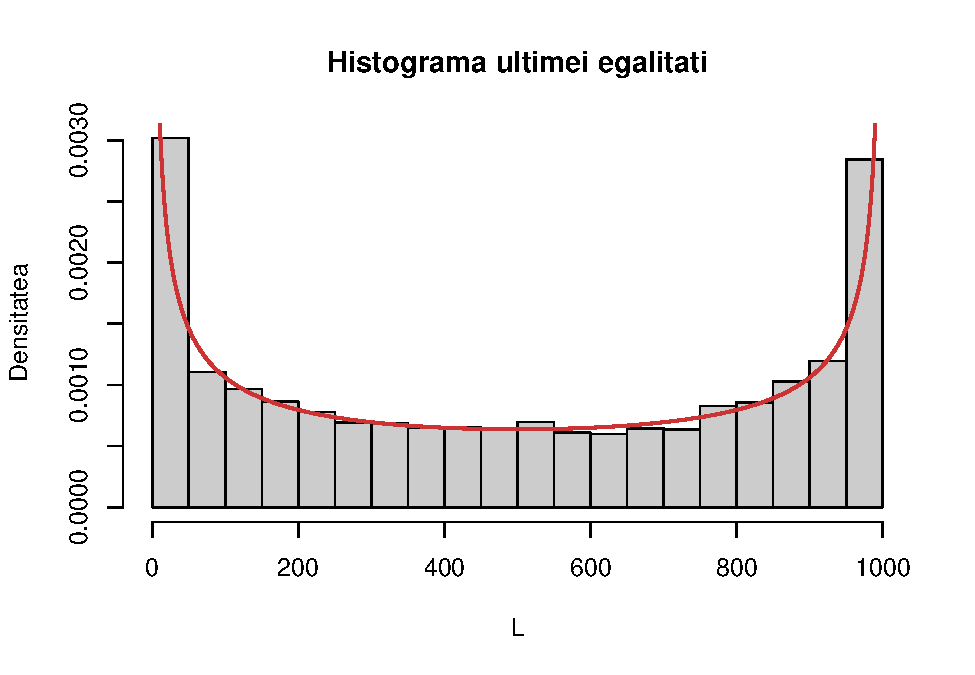
\includegraphics{Lab_Suplimentar_files/figure-latex/unnamed-chunk-19-1} \end{center}


\end{document}
